\chapter{Arquitetura para compartilhamento de informações do ativo}
\label{cha:arquitetura}
	
	A elaboração de uma arquitetura comum para o compartilhamento de informações do ativo é essencial para que haja consistência e interoperabilidade entre os membros da Cadeia de Suprimentos (CS) adotando este sistema.
	
	Este capítulo tem o objetivo de apresentar detalhes da arquitetura proposta baseada em \textit{Web Services} (WS) nos modelos de uma arquitetura orientada a serviços (SOA) compatível com Componentes I4.0 para o compartilhamento de informações do ativo ao longo da CS. A fins de simplificação do texto, os \textit{Web Services} serão mencionados apenas como ``serviços''.
	
	Neste capítulo, é apresentado também o mapeamento dos componentes desta arquitetura dentro do eixo camadas do RAMI4.0.
	
\section{Componentes e operações de serviços dos AASs}

	Os serviços no escopo desta arquitetura são representações das funcionalidades dos Componentes I4.0 e são fornecidos e consumidos entre \textit{Asset Administration Shells} (AASs).
	
	A lógica de fornecimento e consumo de serviços proposta para a I4.0 segue os moldes de um \textit{Web Service} apresentado na \autoref{sec:webservices}, apresentando os componentes e operações (vide \autoref{fig:componentes-webservice}) adaptados ao AAS.
	
	Esta arquitetura envolve três componentes (atores) básicos: O AAS cliente, o AAS servidor e o AAS repositório; e três operações: publicação, busca e interação.

	Os serviços disponibilizados remotamente pelo AAS servidor escuta e responde solicitações de clientes por meio de uma determinada rede e porta. Os AAS clientes, por sua vez, consomem o serviço disponibilizado pelo servidor por meio de solicitações.
	
	Nesta seção são apresentados detalhes sobre os componentes e operações necessárias para o fornecimento serviços no mundo conectado da I4.0
	
\subsection{Componentes}

	Os componentes da arquitetura e suas inter-relações são apresentados na \autoref{fig:aas-wb}.
	
	\begin{figure}[htb]
		\centering
		\caption{Componentes e operações do WS.}
		\label{fig:aas-wb}
		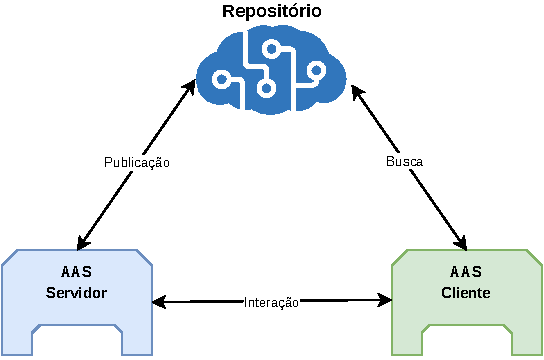
\includegraphics[width=0.7\textwidth]{aas-wb}
		\fonte{O autor.}
	\end{figure}

	De maneira sucinta, os componentes são descritos da seguinte forma: ``O AAS Servidor'' é a parte que possui um serviço a oferecer para os demais AASs no mundo conectado, o ``AAS Cliente'' é a parte que necessita de um serviço e que age ativamente para receber este serviço e o ``AAS Repositório'' é a parte que armazena informações sobre descrições de diversos serviços.
	
	A \autoref{tab:componentes-ws} lista os componentes da arquitetura para a I4.0 e suas respectivas descrições detalhadas.
	
	\begin{table}[htb]
		\centering
		\caption{Componentes da arquitetura para a I4.0.}
		\label{tab:componentes-ws}
		\begin{tabular}{p{3cm}p{12cm}}
			\hline
			\textbf{Componente}
			& \textbf{Descrição} \\ 
			
			\hline
			AAS Servidor
			& O AAS Servidor é a conexão direta com o ativo. Este AAS extrai e disponibiliza informações sobre seu ativo para sua própria MDP. Cada submodelo do AAS representa um conjunto de informações e serviços semelhantes agrupados. \\
			
			\hline
			AAS Cliente
			& O AAS Cliente é a parte que irá consumir as informações disponibilizadas pelo AAS Servidor. O cliente representa cada uma das partes envolvidas na cadeia de suprimentos. Pode representar uma instituição, uma pessoa física ou até mesmo uma outra máquina/produto. \\
			
			\hline
			AAS Repositório
			& O repositório é a plataforma que recebe, armazena e disponibiliza informações de descrição sobre todos os serviços disponíveis no mundo conectado. O AAS recebe operações de ``publicação'' por parte do AAS Servidor e operações de ``busca'' por parte do AAS Cliente. O Repositório não atua como canal de comunicação entre AAS Cliente e Servidor, mas apenas fornece informações necessárias para que ambos os AAS possam se comunicar diretamente por meio da operação de ``interação''. \\
			
			\hline
		\end{tabular}
		\fonte{O autor.}
	\end{table}
	
	Neste modelo, a descrição dos serviços disponíveis nos submodelos de cada AAS é armazenada em um repositório comum, onde todos os AASs disponíveis no mundo conectado na I4.0 poderiam se tornar visíveis. A função do repositório é armazenar uma descrição dos serviços disponíveis e não o serviço em si. O serviço é fornecido pelo próprio AAS que o disponibilizou, servindo o repositório apenas como uma plataforma de descobertas de serviços.

	Cada AAS pode atuar tanto como um fornecedor de serviços (servidor), quanto como um solicitante de serviços (cliente), ou como ambos. Sempre usando o repositório como plataforma para descoberta.

\subsection{Operações}
	As operações de serviços de AASs e suas inter-relações com os componentes são mostradas por meio dos arcos na \autoref{fig:aas-wb} e suas descrições detalhadas são apresentadas na \autoref{tab:operacoes-ws}
	
	\begin{table}[htb]
		\centering
		\caption{Operações do WS para I4.0.}
		\label{tab:operacoes-ws}
		\begin{tabular}{p{3cm}p{12cm}}
			\hline
			\textbf{Operação}
			& \textbf{Descrição} \\ 
			
			\hline
			Publicação
			& Ação tomada pelo AAS Servidor sempre que este componente queira anunciar um serviço para que possa ser descoberto. Nesta operação, o AAS Servidor envia uma lista de seus serviços ofertados e a descrição de cada um desses serviços. Esta lista é recebida e armazenada pelo Repositório, que a disponibiliza para acesso público. \\
			
			\hline
			Busca
			& Ação tomada pelo AAS Cliente sempre que este precisa consultar serviços de seu interesse. Nesta operação o AAS Cliente faz uma solicitação ao Repositório com os parâmetros que definem o tipo e as restrições do serviço desejado. A operação de busca engloba também o fluxo contrário de informações, que é o envio da resposta da solicitação do Repositório para o AAS Cliente. \\
			
			\hline
			Interação
			& Ação tomada pelo AAS Cliente sempre que este deseja invocar um serviço. O AAS Cliente estabelece uma conexão direta com o AAS Servidor e consome o determinado serviço solicitado. A operação de interação normalmente é feita após o recebimento da lista de descrição de serviços por parte do Repositório, porém a interação pode ser feita diretamente caso o AAS Cliente já possua informações necessárias para o estabelecimento da conexão.  \\
			
			\hline
		\end{tabular}
		\fonte{O autor.}
	\end{table}

	Para cada uma das operações, deve ser definido também o WSD (\textit{Web Services Description}), documento o qual estabelece os padrões de comunicação suportados pelo AAS Servidor, como, por exemplo, o padrão REST ou o padrão SOAP; e especifica como acessar e quais as operações ou métodos estão disponíveis no serviço. 
	
	Quando o AAS atua como Servidor, este publica a descrição de seus serviços no repositório por meio de uma API (\textit{Application Programming Interface}) definida no WSD. Quando como Cliente, o AAS busca no repositório um serviço desejado e recebe uma lista de opções de serviços com suas respectivas descrições~. Assim, o serviço mais adequado pode ser selecionado.
	
	Uma vez definido o serviço a ser consumido, o AAS Cliente estabelecerá a conexão direta com o AAS Servidor por meio de algum dos padrões suportados, utilizando os detalhes contidos na descrição do serviço para localizar, contactar e invocar o serviço.	
	
	A \autoref{fig:pfs-ws} apresenta um diagrama PFS (\textit{Production Flow Schema}) com o fluxo ocorrência das operações básicas no WS para a I4.0.
	
	\begin{figure}[htb]
		\centering
		\caption{Diagrama PFS das operações do WS.}
		\label{fig:pfs-ws}
		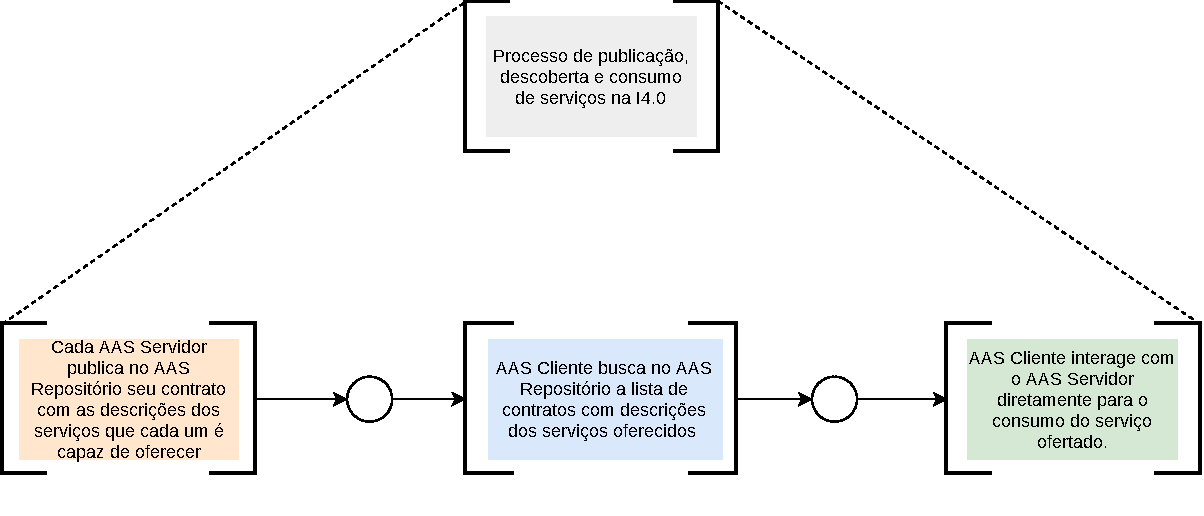
\includegraphics[width=1\textwidth]{pfs-ws}
		\fonte{O autor.}
	\end{figure}
	
	Os serviços fornecidos por um AAS são diversos. Entretanto, neste trabalho serão tratados com ênfase aqueles serviços que têm como objetivo o compartilhamento de informações sobre o ativo que possam agregar valor ao produto ao longo de sua cadeia de suprimentos. Ou seja, os serviços que extraem informações da MDP do AAS e as fornecem, mediante autenticação, às partes solicitantes ao longo da cadeia de suprimentos.

\section{Estrutura do AAS }

	Nesta proposta de arquitetura de WS, o conceito de Memória Digital do Produto (MDP) é inserido dentro da Indústria 4.0 com o objetivo de se agregar valor ao produto por meio da possibilidade de acesso a informações sobre o ativo entre parceiros ao longo da cadeia de valor.
	
	Nesta seção são apresentados os detalhes sobre uma possível estruturação do AAS para que seja compatível com a proposta de fornecimento de WSs.
	
\subsection{Integração da MDP ao AAS}

	A MDP precisa ser integrada ao AAS para que possa ter a estrutura necessária para que seus dados sejam disponibilizados ao mundo conectado da I4.0. A MDP em um AAS corresponde aos dados do ativo, ao gerenciamento desses dados e às funções básicas aplicadas em cima desses dados. A MDP contém informações referentes a cada um dos submodelos em um AAS. Cada submodelo agrega informações semelhantes relativas ao ativo. 
	
	A MDP, na pratica, não estará necessariamente presente no escopo físico do ativo ao qual ela se relaciona. Como a MDP é parte integral do AAS, que representa a parte virtual do ativo, esta pode ser fornecida em qualquer meio digital, inclusive em plataformas de serviços de computação em nuvem. Estas plataformas específicas suportam o armazenamento de grandes quantidades de dados, assim como podem assegurar uma alta capacidade de processamento requisições de serviços solicitados.
	
	As informações contidas na MDP devem ser estruturadas de forma tal que facilite a interpretação destes dados do lado do cliente. Para isso, metamodelos devem ser aplicados. Os metamodelos estabelecem os moldes sobre o qual devem ser elaborados os dados.
	
	\citeonline{bader2019aas} estabelece padrões de metamodelos para a implementação de submodelos no AAS, porém não aborda um possível repositório de serviços e o armazenamento de descrições de serviços. A \autoref{tab:mdp-repositorio} traz uma proposta de metamodelo para a MDP do AAS Repositório para o armazenamento de descrições de serviços.
	
	\begin{table}[htb]
		\centering
		\caption{Proposta de metamodelo para a MDP do repositório.}
		\label{tab:mdp-repositorio}
		\begin{tabular}{p{3cm}p{12cm}}
			\hline
			\textbf{Propriedade}
			& \textbf{Descrição} \\ 
			
			\hline
			ID do AAS provedor
			& Tem a função de distinguir exclusivamente os AAS e todos seus elementos \cite{adolphs2016structure} no mundo conectado da I4.0. Alguns tipos possíveis de identificadores são \cite{bader2019aas}: IRDI, IRI e UUID. \\
			
			\hline
			ID do serviço
			& Identificação exclusiva do serviço para a sua identificação única entre todos os repositórios. \\
			
			\hline
			Descrição do AAS provedor
			& Breve descrição sobre o AAS servidor \\
			
			\hline
			Protocolo de comunicação
			& Protocolos de comunicação suportados pelo fornecedor daquele serviço, como, por exemplo, HTTP, MQTT, etc.  \\
			
			\hline
			Especificações do protocolo
			& Padrão de especificação para a comunicação, como, por exemplo, REST, SOAP, etc. \\
			
			\hline
			Formato de intercâmbio
			& Formato de arquivo de intercâmbio de informações. Ex.: json, xml, yaml, aasx, etc.  \\
			
			\hline
			Data de inserção
			& Data de inserção do serviço ao Repositório. \\
			
			\hline
			Está ativo?
			& Chave booleana indicando se o AAS servidor atualmente suporta requisições.  \\
			
			\hline
			Tempo resposta
			& Tempo médio dinâmico de resposta do serviço baseado no tempo de resposta observado por diversas requisições executadas. \\
			
			\hline
			Índice de reputação
			& Índice para mensuração da qualidade do serviço prestado. Baseado em avaliações de AAS clientes que já consumiram o serviço.  \\
			
			\hline
			Descrição do serviço
			& Descrição sobre o funcionamento do serviço juntamente com o tipo de resposta esperado.  \\			
			\hline
		\end{tabular}
		\fonte{O autor.}
	\end{table}
	
	A \autoref{tab:mdp-repositorio} é uma lista não exaustiva das propriedades necessárias para o armazenamento de um serviço, ela apenas apresenta uma ideia sobre os tipos de chaves básicas necessárias para identificação e invocação de um serviço na rede.
	
	O AAS Cliente na operação de busca fará uma requisição ao repositório ou a um lista de repositórios e receberá (de cada um dos repositórios) por meio de uma API a lista de serviços com uma estrutura de dados contendo os atributos chave-valor mencionados na \autoref{tab:mdp-repositorio}.
	
	Já o metamodelo da MDP do AAS servidor possuirá uma estrutura diferente, uma vez que deverá possuir as funções de agregação necessárias para a geração de alguns atributos. Uma proposta de metamodelo para a MDP do AAS servidor é apresentada na \autoref{tab:mdp-servidor}.
	
	\begin{table}[htb]
		\centering
		\caption{Proposta de metamodelo para a MDP do servidor.}
		\label{tab:mdp-servidor}
		\begin{tabular}{p{4cm}p{11cm}}
			\hline
			\textbf{Propriedade/Função}
			& \textbf{Descrição} \\ 
			
			\hline
			ID do serviço
			& Identificação exclusiva do serviço para a sua identificação única entre todos os repositórios. \\
			
			\hline
			Extração de dados dos submodelos
			& Função que retorna os dados solicitados pelo serviço. \\
			
			\hline
			Pré-processamento dos dados
			& Pré-processamento e limpeza dos dados brutos extraídos dos submodelos. \\
			
			\hline
			Atualização do tempo de resposta
			& Função de atualização do tempo médio de resposta do serviço com base em solicitações já respondidas. \\
			
			\hline
			Cálculo do índice de reputação
			& Função para cálculo e armazenamento do índice de reputação com base nas avaliações de AAS clientes que já consumiram o serviço. \\
			
			\hline
			Atualização da descrição do serviço no repositório
			& Envia aos repositórios listados uma atualização das descrições dos serviços. \\
			
			\hline
			Repositórios
			& Lista de repositórios onde o serviço está visível. \\			
			\hline
		\end{tabular}
		\fonte{O autor.}
	\end{table}
	
	A \autoref{tab:mdp-servidor}, assim como os metamodelos da MDP do Repositório, faz uma listagem não exaustiva de suas propriedades, sendo possível a inserção de novas funcionalidades adicionais na implementação do AAS. O metamodelo proposto na tabela se relaciona às funções da MDP em gerar a descrição dos serviços. Além desta atividade, a MDP possui as funções convencionais de armazenamento e gerenciamento dos dados dos submodelos, não contempladas pelo metamodelo. 
	
	Com a MDP, o AAS servidor será, portanto, o único responsável pela geração e atualização de todos os metadados referentes aos serviços de seu AAS.

	
\subsection{ Detalhamento das partes do AAS }

	Nesta subseção é apresentada uma proposta de detalhamento da estrutura do AAS contendo todas as partes necessárias para a implementação da arquitetura de compartilhamento de serviços baseada no RAMI4.0. 
	
	A estrutura proposta do AAS é baseda em \citeonline{bader2019aas}, que estabelece a divisão do AAS em submodelos e o divide em duas partes: o cabeçalho (\textit{header}) e o corpo (\textit{body}).
	
	O cabeçalho na estrutura proposta terá a função de providenciar informações públicas sobre o ativo que o identifiquem minimamente e que forneça uma descrição sobre seus serviços oferecidos. O cabeçalho deverá conter informações que podem ser acessadas sem a necessidade de autenticação, como, por exemplo, seu identificador único universal (UUID - \textit{Universal Unique IDentifier}), o modelo e fabricante do ativo. O cabeçalho deverá conter também a descrição dos serviços fornecidos por seus submodelos. A descrição dos serviços é enviada ao repositório ou pode ser também consultada diretamente pelo AAS solicitante.
	
	A descrição de cada serviço em um cabeçalho de AAS deverá necessariamente conter também referências ao AAS Servidor, ou seja, \textit{links} e identificações que permitam que o cliente possa localizar, contactar e invocar o serviço ofertado.
	
	O cabeçalho não terá a função de fornecer uma ficha técnica detalhada, mas apenas uma caracterização abstrata do ativo. Dependendo da confidencialidade do ativo, o submodelo de identificação pode apenas apresentar o UUID como informação pública. Sem o UUID, o AAS se torna inacessível para qualquer uma das partes da cadeia de suprimentos.
	
	Dentro dos moldes da estrutura proposta, o corpo (\textit{body}) de um AAS fornece as informações e funcionalidades sensíveis sobre o ativo, que podem ser acessadas mediante autenticação. As funcionalidades dos ativos são agrupadas em forma de submodelos, conforme estabelecido em \citeonline{bader2019aas, adolph2018roadmap, bedenbender2017aasexamples}, que são unidades de agrupamento de funcionalidades semelhantes, como propriedades, serviços e demais regras de negócio do ativo. Já os dados relativos aos submodelos são armazenadas e gerenciadas pela MDP, que também está localizada no corpo do AAS.
	
	O corpo do AAS representa a carga útil (\textit{payload}) do AAS, pois é a porção de informação que é de fato relevante para o cliente que consumirá os serviços ofertados.
	
	A estrutura de um AAS compatível com a arquitetura orientada a serviços proposta é apresentada na \autoref{fig:estrutura-aas}.
	
	\begin{figure}[htb]
		\centering
		\caption{Estrutura do AAS com seus submodelos e a MDP.}
		\label{fig:estrutura-aas}
		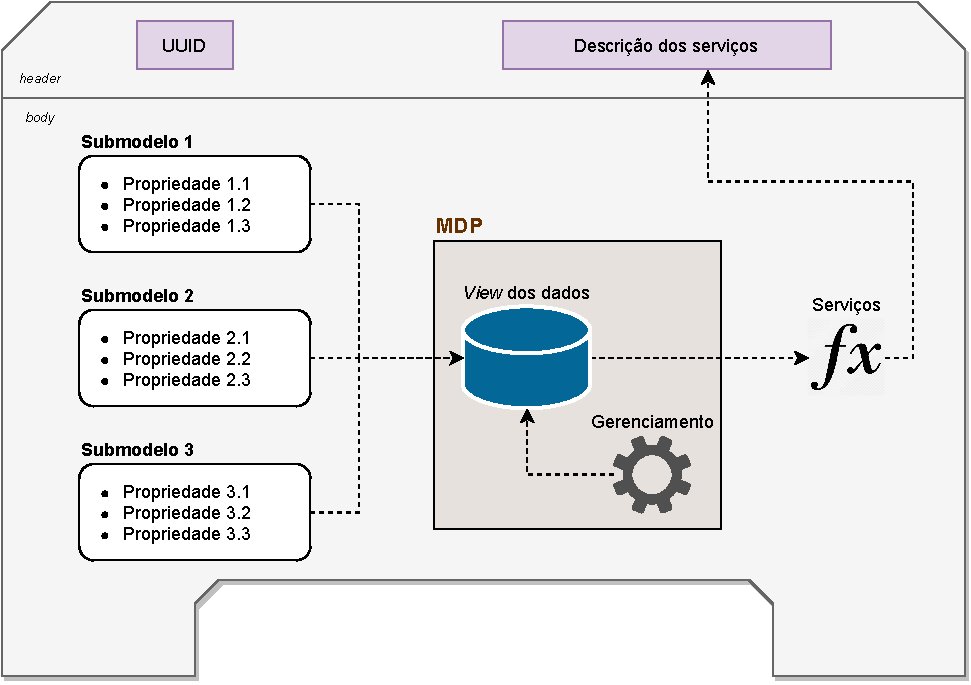
\includegraphics[width=0.7\textwidth]{estrutura-aas}
		\fonte{O autor.}
	\end{figure}

	Os dados contidos na MDP sobre submodelos, quando processados, fornecem informações sobre o ativo e agregam valor ao mesmo. Além disso, novos modelos de negócio surgem sob os dados gerados pelo ativo.
	
	Neste trabalho, é dado enfoque aos submodelos que oferecem serviços de consulta de dados a qualquer uma das partes ao longo da cadeia de suprimentos. Alguns exemplos desse tipo de submodelo podem incluir: a ficha técnica detalhada do ativo, submodelos de histórico de leitura de sensores, histórico de geolocalização do ativo, histórico de padrão de uso, etc.


\section{Fluxo de fornecimento de serviços}

	As etapas para o fornecimento de serviços na I4.0 segue um fluxo padrão. A \autoref{fig:wb-funcionamento} demonstra uma exemplificação do fluxo de operações básicas de um WS em funcionamento. Neste exemplo, o AAS de um produto \textbf{(a)} mantém contato com o AAS da empresa do fabricante \textbf{(b)}, com o AAS da empresa do distribuidor \textbf{(c)} e com o AAS do consumidor final \textbf{(d)}, fornecendo o serviço de consulta de informações de diferentes submodelos para cada um dos solicitantes. 	
	
	\begin{figure}[htb]
		\centering
		\caption{Exemplificação das operações de publicação e busca.}
		\label{fig:wb-funcionamento}
		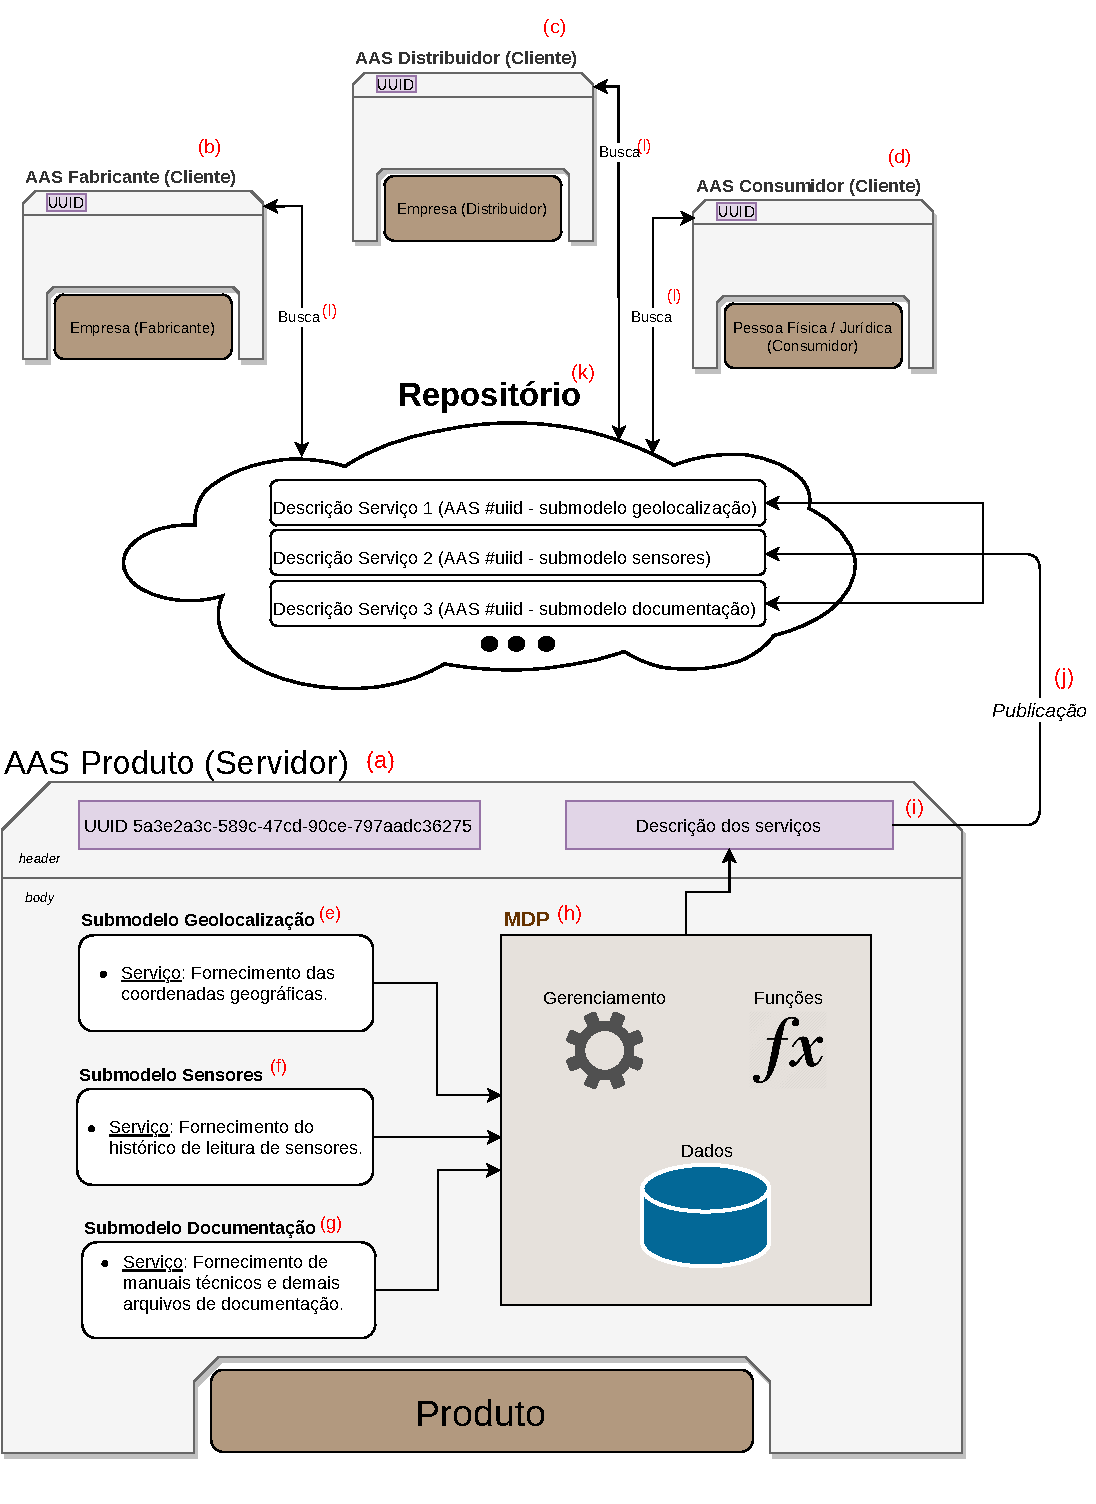
\includegraphics[width=0.8\textwidth]{wb-funcionamento}
		\fonte{O autor.}
	\end{figure}

	Neste exemplo há três submodelos disponíveis no AAS Produto: Submodelo ``geolocalização'' \textbf{(e)}, submodelo ``sensores'' \textbf{(f)} e submodelo ``documentação'' \textbf{(g)}. Os serviços de todos os submodelos disponíveis são mapeados pelas funções da MDP \textbf{(h)} e, assim, é gerada uma lista de descrições de serviços \textbf{(i)}. Esta lista de descrições de serviços é publicada \textbf{(j)} no repositório.
	
	O repositório \textbf{(k)} recebe a descrição de serviços do AAS Produto e as disponibiliza para consulta. O repositório receberá também listas de descrição de serviços de diversos outros AASs.
	
	Os AAS Clientes fazem a busca \textbf{(l)} no repositório. As buscas são feitas com parâmetros a fim de se restringir qual tipo de serviço aquele cliente pretende consumir, podendo-se restringir a busca, inclusive, ao serviço de um AAS específico, identificando-o por meio de seu UUID.
	
	Cada AAS Cliente (Fabricante, Distribuidor ou Consumidor), portanto, realiza a consulta ao repositório com os seus parâmetros de interesse e recebe a resposta com descrições detalhadas sobre os serviços disponíveis e informações para localizar, contactar e invocar estes serviços.
	
	O próximo passo após o recebimento da resposta do repositório é a decisão interna de cada AAS Cliente sobre qual serviço selecionar. Uma vez definido, o AAS Cliente estabelece uma comunicação direta com o AAS Servidor para o consumo do serviço selecionado.
	
	Este é um exemplo de consulta única. Em aplicações reais, o cliente normalmente invocaria o serviço de diversos AAS Servidores ao mesmo tempo, como, por exemplo, um fabricante solicitando informações de todas as máquinas de um modelo específico que foram vendidas a clientes espalhados pelo mundo para se realizar análise de dados a fim de se fazer uma manutenção preditiva por meio da identificação de potenciais falhas.
	
	Todas as atividades de invocação de serviços na fase de interação são feitas mediante autenticação. É responsabilidade das funções da MDP realizar a autenticação ou bloqueio dos serviços disponíveis de acordo com as políticas de acesso de cada AAS.
	
	É importante notar que no mundo da I4.0 todo ativo é englobado por um AAS e se torna um Componente I4.0. Como o repositório detém informações e funções que agregam valor ao negócio, este pode também ser considerado um ativo e, portanto, possui o seu próprio AAS, que é responsável por toda a parte virtual deste ativo.
	
\section{Mapeamento das operações no RAMI4.0}
	
	Segundo \citeonline{iec2017rami}, o RAMI4.0 fornece uma visão estruturada dos principais elementos de um ativo usando um modelo de níveis composto por três eixos. Desta forma, inter-relações complexas podem ser divididas em seções menores e mais gerenciáveis, combinando os três eixos para representar cada aspecto relevante do estado do ativo em cada ponto de seu ciclo de vida.
	
	Esta seção tem o objetivo de mapear as operações do WS para dentro das camadas do RAMI4.0 de forma a representar todas as etapas do fluxo de informações em um modelo unificado.
	
	O mapeamento para o RAMI4.0, que é uma arquitetura de referência para a I4.0, contribui também para facilitar a execução de implementações do modelo de WS junto a outras soluções de I4.0, garantindo a interoperabilidades entre os sistemas.

\subsection{Descrição das camadas do RAMI4.0}

	Na \autoref{sub:rami4} são apresentados os detalhes do RAMI4.0 e o detalhamento de cada nível do eixo Camadas com suas funções gerais. Aqui é apresentada novamente cada camada do eixo Camadas dando o enfoque para suas funções específicas para as operações de um WS.

	A camada mais inferior, \textbf{Ativo} é onde estará o elemento real do Componente I4.0 como, por exemplo, máquinas, sensores, pessoas, etc; e qualquer outro elemento, físico ou não, que represente valor ao negócio. O ativo será a fonte de dados, os quais serão compartilhados por meio de serviços para as partes ao longo da cadeia de suprimentos.
	
	Para a ideia de compartilhamento de informações no mundo I4.0, os dados a serem extraídos do ativo são estrategicamente selecionados como o objetivo de reunir somente os dados que possam agregar valor ao próprio ativo. Assim, estes dados selecionados são extraídos do ativo e repassados às camadas superiores até que cheguem à Camada de Informação, onde são armazenados na MDP.
	
	Cada elemento desta camada, os ativos, deve possuir meios de comunicação e identificadores únicos (UUID), para permitir o seu monitoramento e supervisão dos dispositivos de controle por meio do AAS \cite{adolphs2015rami}.
	
	Na arquitetura orientada a serviços é possível elencar alguns componentes importantes para essa camada, como os dispositivos físicos e sensores. Outros elementos usuais dessa camada como os dispositivos de atuação e de controle também estariam inclusos, porém não são responsáveis pela extração de dados.
	
	Na camada de \textbf{Integração} estão as funcionalidades convencionais responsáveis pela virtualização de todos os ativos da camada inferior \cite{adolphs2015rami}. Representa a ponte entre o mundo real e o virtual.
	
	Na arquitetura proposta para o compartilhamento de informações do ativo, esta camada está presente no AAS Servidor, pois é dele que serão extraídos os dados desde o ativo até as camadas superiores, tanto o AAS Cliente quanto o AAS Repositório já operam nas camadas virtuais. Esta camada adotará alguma tecnologias de transferência de dados consolidada como, por exemplo, o Wi-Fi, Ethernet, 5G, Bluetooth, etc.
	
	A camada \textbf{Comunicação} estabelecerá o protocolo de comunicação OPC UA para o AAS Servidor se comunicar com as camadas superiores. É feito o pré-processamento de dados nesta fase, ou seja, antes de ser enviado para a camada de informação, onde será salvo na MDP. O pré-processamento dos dados incluirá a remoção de redundâncias, duplicidades e remoção de \textit{outliers}.
	
	A camada de \textbf{Informação} é onde os dados são de fato armazenados, para isso, modelos de estrutura de Banco de Dados (BD) são definidos de acordo os tipos de dados e suas aplicações. Alguns exemplos de estrutura de dados incluem: BDs relacionais (e.g., MySQL, Postgres, SQLite) \cite{morris2017relationaldatabase} e demais BDs NoSQL como os orientados a documentos (e.g., MongoDB, CouchDB), os do tipo chave-valor (e.g., Redis, DynanoDB), os de armazenamento em coluna ampla (e.g., Cassandra, HBase) e os baseados em grafos (e.g.,Neo4j, JanusGraph) \cite{schaefer2019nosql}.
	
	Desta forma, esta camada é responsável por gerar e armazenar a descrição dos serviços oferecidos pelo AAS Servidor. Além disso, esta camada contém a parte da MDP realiza a autenticação dos AAS solicitantes, ou seja, realiza o controle de acesso a suas informações.
	
	Na camada \textbf{Funcional} é onde ocorre toda a interação horizontal com outros AASs contidos no mundo conectado da I4.0. Esta camada é responsável pela integração horizontal entre as partes da cadeia de suprimentos de um produto. Os serviços são disponibilizados por meio da camada funcional, portanto é a interface entre os AASs. 
	
	Esta camada define o tipo de protocolo a ser utilizado para o fornecimento dos \textit{Web Services}, o protocolo HTTP é o mais comumente adotado para o fornecimento de WSs \cite{gruner2016restful}. Qualquer outro protocolo de aplicação também pode ser adotado como, por exemplo, o MQTT \cite{yokotani2016mqtt}.
	
	A última camada, \textbf{Regra de Negócio}, é onde estão contidas as questões legais do AAS, como as políticas de privacidade dos dados, as condições regulatórias \cite{adolphs2015rami}. No contexto da arquitetura de compartilhamento baseada em \textit{Web Services}, esta camada conterá as restrições aplicadas sobre os serviços, como as políticas de privacidade de dados e as regras relacionadas às restrições de acesso a determinados serviços.
	
	Para os WSs, outra função importante desta camada é a orquestração dos serviços, que se refere ao gerenciamento dos serviços oferecidos. Quando os serviços são oferecidos em forma de contêineres, o orquestrador de serviços permite a escalabilidade da capacidade de trabalho, permitindo a invocação ou remoção de contêineres de acordo com a demanda de um determinado serviço. Alguns orquestradores de contêineres podem ser citados, como o Kubernetes, Docker Swarm e Apache Mesos \cite{redhat2020orchestration}.
	
	O conjunto de todas estas camadas representa um \textbf{Componente I4.0}. Para cada tipo de operação relacionada a um componente, é necessário detalhar o fluxo de dados e de eventos acontecendo em cada uma das camadas. Este detalhamento permite que implementações de soluções I4.0 sejam facilitadas e garante que a criação dessas soluções por diversos desenvolvedores de sistemas resulte em sistemas que sejam interoperáveis, independentemente da tecnologia adotada.
	
	O \textbf{Componente I4.0} pode ainda ser mais detalhadamente especificado, identificando se o componente representa um produto em desenvolvimento ou uma instância de um produto já fabricado. Estas considerações são cobertas pelo eixo Ciclo de Vida e Cadeia de Valor e considerações sobre este eixo envolvendo a arquitetura proposta baseada em WSs será apresentada no \autoref{cha:ciclo-de-vida}.
	
	A \autoref{fig:wb-rami} apresenta os componentes da arquitetura de fornecimento de WSs dentro do eixo Camadas do RAMI4.0, que são:
	
	\begin{itemize}
		\item \textbf{Ativo}: Dispositivos de campo, sensoriamento; 
		\item \textbf{Integração}: Virtualização, protocolos de transferência de dados; 
		\item \textbf{Comunicação}: Pré-processamento de dados e protocolos de comunicação; 
		\item \textbf{Informação}: Controle de acesso e autenticação, análise de dados, armazenamento, descrição dos serviços;
		\item \textbf{Funcional}: serviços, protocolos de aplicação, interface entre AASs; 
		\item \textbf{Regra de negócio}: Orquestração de serviços, políticas de privacidade e condições regulatórias.
	\end{itemize}
	
	\begin{figure}[H]
		\centering
		\caption{Camadas do RAMI4.0 com os componentes da arquitetura.}
		\label{fig:wb-rami}
		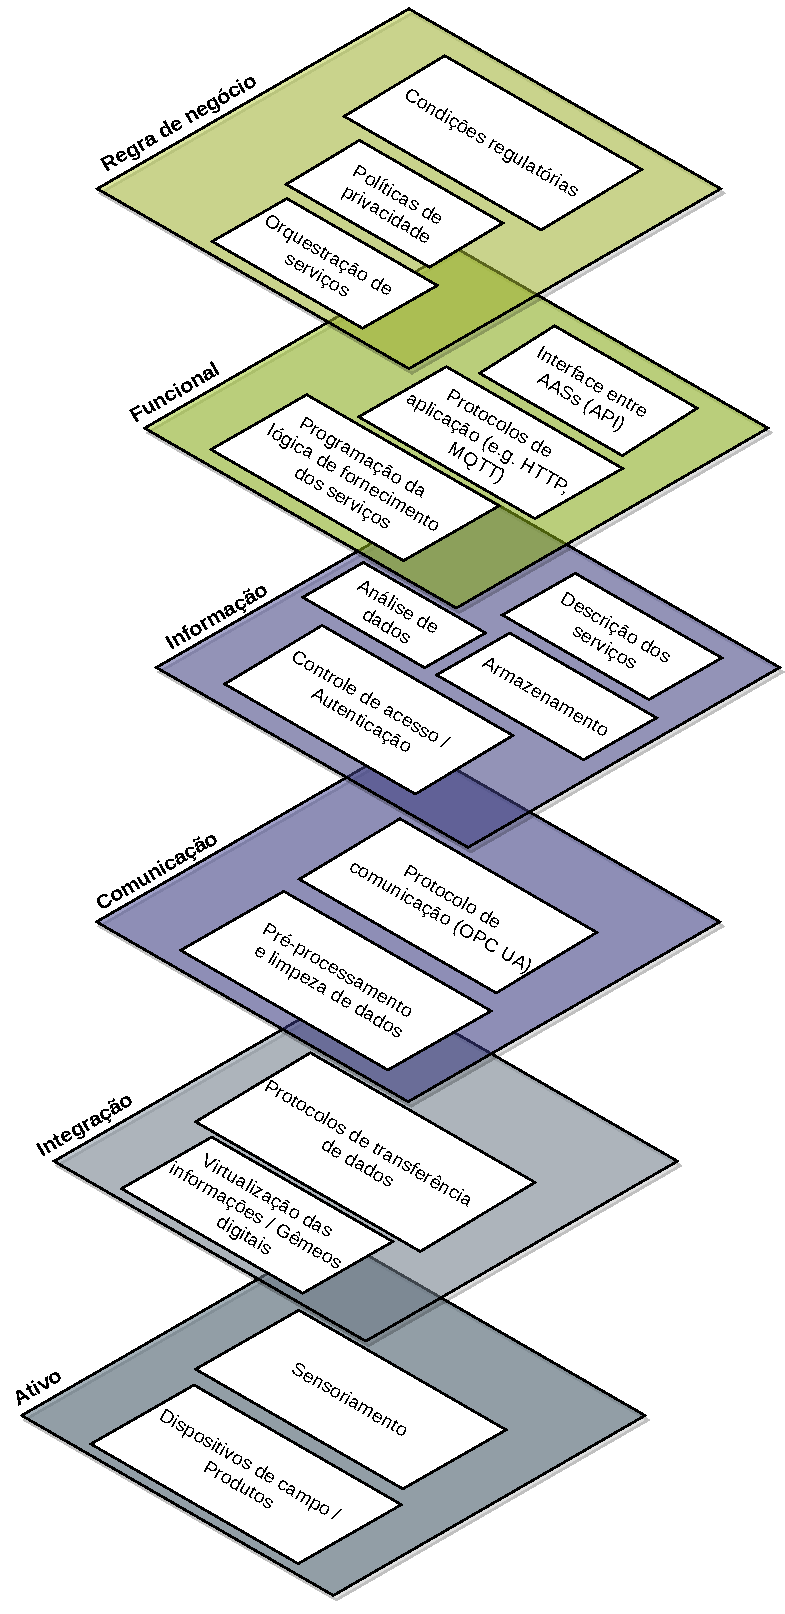
\includegraphics[height=0.9\textheight]{wb-rami}
		\fonte{O autor.}
	\end{figure}

\subsection{Operação de Publicação}

	A \autoref{fig:rami-publicacao} apresenta diagramas PFS do fluxo de atividades para a operação de publicação de um AAS Servidor em um Repositório.
	
	\begin{figure}[htb]
		\centering
		\caption{Diagrama PFS da operação de publicação.}
		\label{fig:rami-publicacao}
		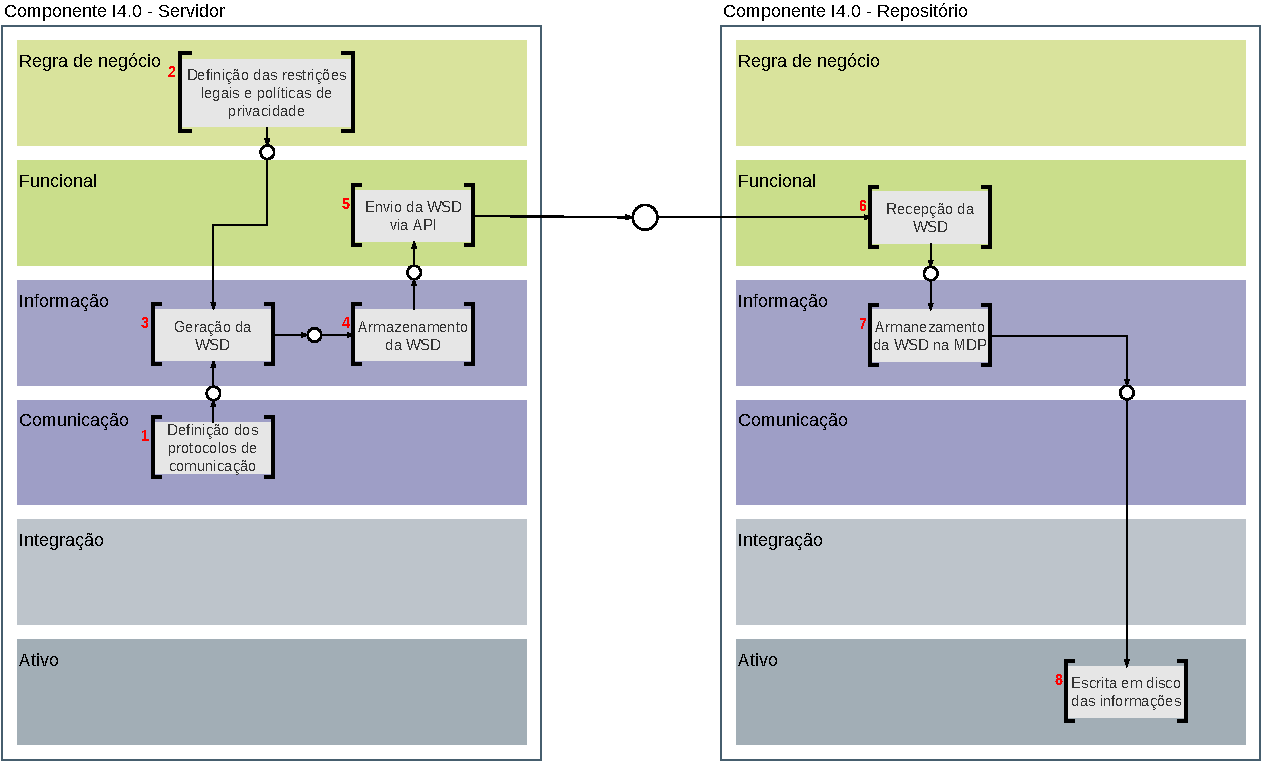
\includegraphics[width=1\textwidth]{rami-publicacao}
		\fonte{O autor.}
	\end{figure}

	Começando pela primeira atividade no Componente I4.0 do Servidor, a descrição do serviço segue um fluxo estabelecido até chegar na MDP do Repositório, os passos são detalhados a seguir:
	
	\begin{enumerate}
		\item A geração da descrição dos serviços é feita com base nos serviços disponíveis na MDP do servidor. Uma descrição de cada serviço ativo é gerada em uma linguagem WSD.
		\item A lista de descrição de serviços é armazenada em sua MDP local e enviada à camada superior para ser transferida ao repositório.
		\item É feita a definição das especificações da comunicação, onde se estabelece o protocolo de comunicação a ser adotado na API (e.g., HTTP, MQTT), assim como o tipo de arquitetura (e.g., REST, SOAP) e o formato de intercâmbio (e.g., json, xml, yaml).
		\item A descrição dos serviços é enviada ao Repositório via API, definida pelas especificações da comunicação.
		\item A descrição dos serviços é recebida pelo Repositório em um formato de intercâmbio definido. A descrição dos serviços nesta fase já contém todas as informações para a identificação do serviço e seu AAS correspondente.
		\item A lista de serviços é armazenada junto aos demais serviços na MDP do Repositório.
	\end{enumerate}

\subsection{Operação de Busca}

	A operação de busca é dividida em duas partes: a requisição e a resposta. A \autoref{fig:rami-busca-requisicao} apresenta diagramas PFS da requisição de um Cliente a um Repositório em uma operação de busca e a \autoref{fig:rami-busca-resposta} apresenta a resposta do Repositório ao Cliente na mesma operação
	
	\begin{figure}[htb]
		\centering
		\caption{Diagrama PFS da requisição em uma operação de busca.}
		\label{fig:rami-busca-requisicao}
		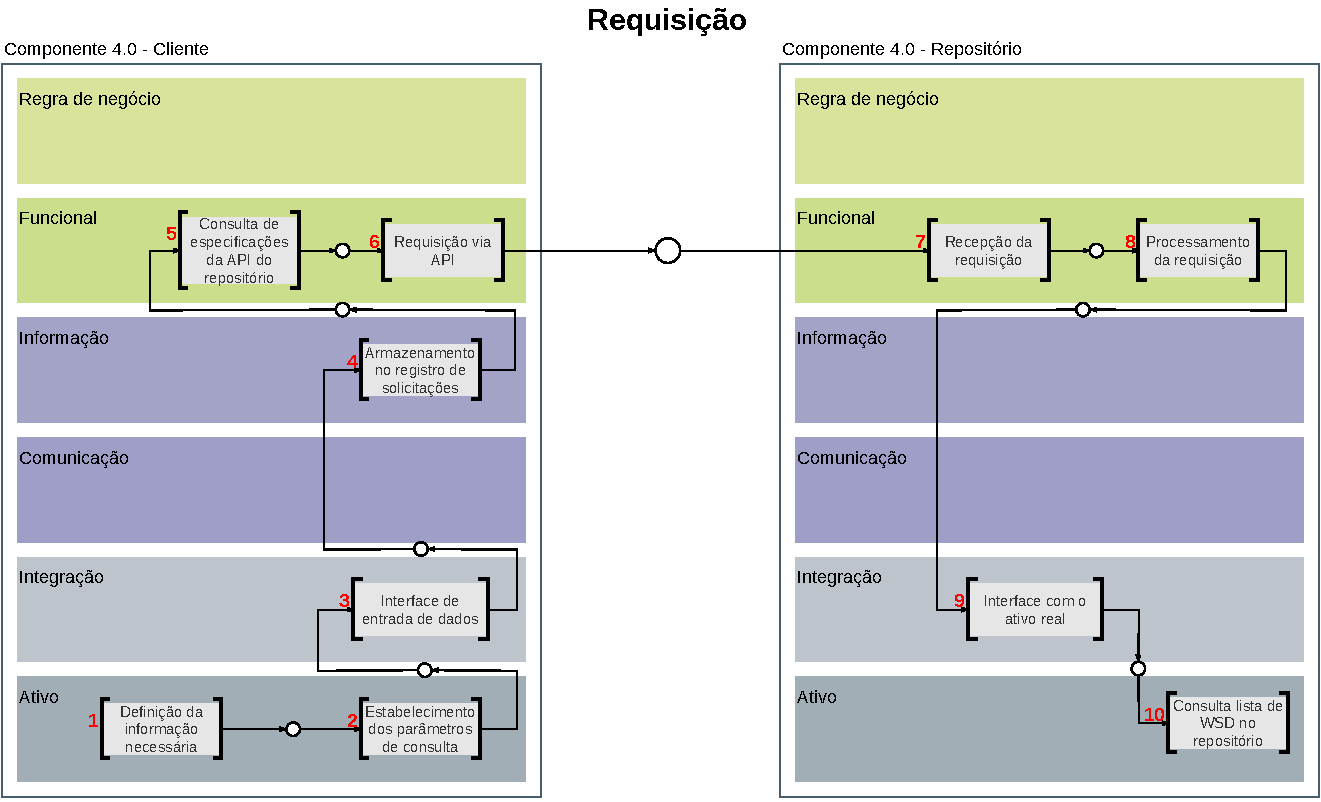
\includegraphics[width=0.9\textwidth]{rami-busca-requisicao}
		\fonte{O autor.}
	\end{figure}

	Começando pela primeira atividade no Componente I4.0 do Cliente, que é a definição dos parâmetros de consulta, a operação de requisição para a busca de um serviço segue um fluxo estabelecido até chegar receber a resposta do Repositório, os passos são detalhados a seguir:
	
	\begin{enumerate}
		\item O processo de requisição começa com a definição dos parâmetros de consulta, que representa o conjunto de restrições que estabelecem qual é exatamente o tipo de serviço que o Cliente deseja consumir. Para os serviços que visam a extração de informações do ativo, os parâmetros representam, por exemplo, o ID do AAS a ser consultado, o horário e data de um determinado evento, uma filtragem por modelos específicos de um produto, etc. Os parâmetros de consulta são estabelecidos pela regra de negócio, isto significa que a regra de negócio diz o que o Componente I4.0 pode ou não consumir, a regra de negócio cria a necessidade de se consumir um serviço sempre que o consumo desse serviço resulte em agregação de valor ao produto/negócio, respeitando-se sempre as demais condições legais e regulatórias.
		\item É feita a definição das especificações de comunicação, onde se estabelece o protocolo de comunicação a ser adotado na API (e.g., HTTP, MQTT), assim como o tipo de arquitetura (e.g., REST, SOAP) e o formato de intercâmbio (e.g., json, xml, yaml).
		\item A requisição é enviada via API, definida pelas especificações da comunicação.
		\item O repositório recebe a requisição do cliente.
		\item A requisição é processada pelo repositório. Identifica-se nesta fase se a requisição é válida e contém todos os parâmetros necessários para a consulta.
		\item Finalmente é feita a consulta à MDP do Repositório utilizando os parâmetros de consulta estabelecidos pelo cliente.
	\end{enumerate}

	Após a requisição, o repositório envia a resposta ao cliente. O fluxo de atividades da resposta é apresenta com diagramas PFS na \autoref{fig:rami-busca-resposta}.

	\begin{figure}[htb]
		\centering
		\caption{Diagrama PFS da resposta em uma operação de busca.}
		\label{fig:rami-busca-resposta}
		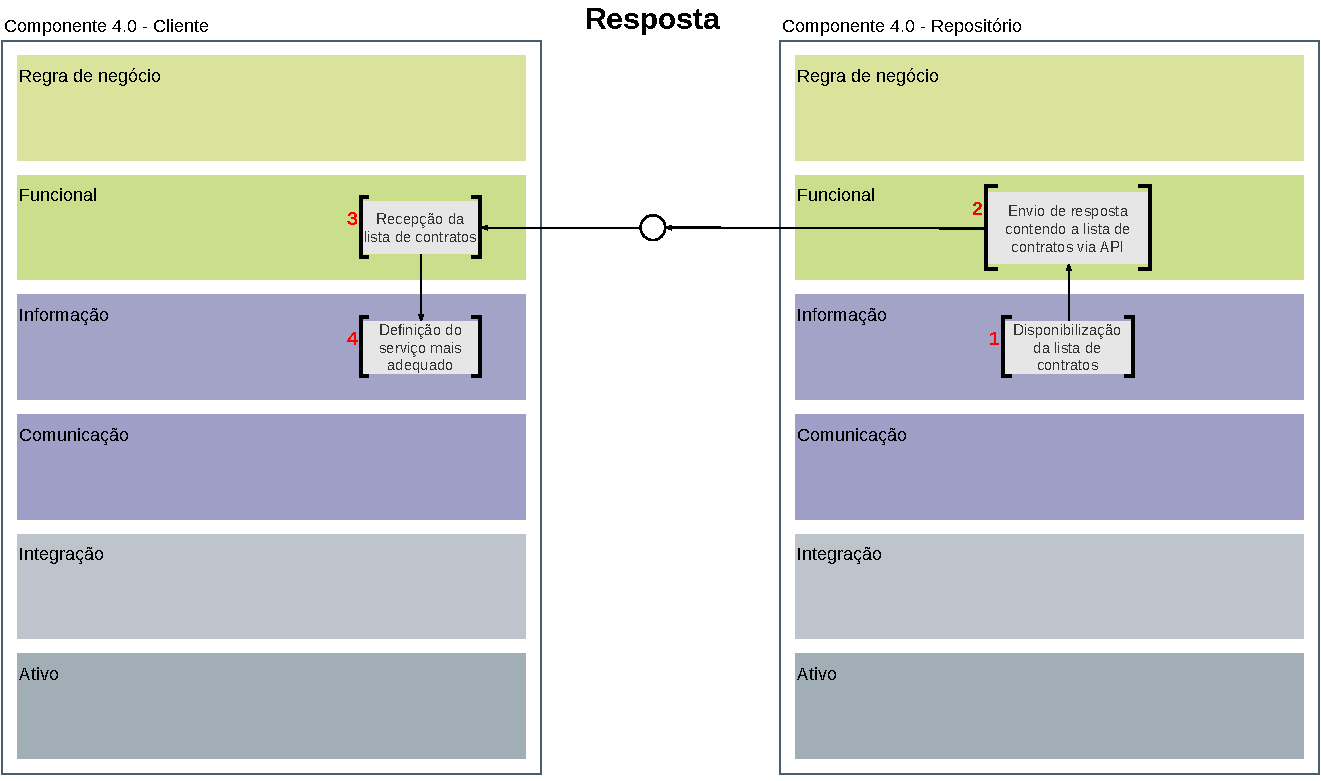
\includegraphics[width=0.9\textwidth]{rami-busca-resposta}
		\fonte{O autor.}
	\end{figure}

	Detalhadamente, a resposta do repositório segue o seguinte fluxo de atividades, começando pela consulta à MDP do repositório à direita:
	
	\begin{enumerate}
		\item A consulta à MDP é realizada e recebe os resultados. Os resultados podem ser uma lista de serviços válidos, assim como podem conter mensagens de erro devido a solicitações inválidas ou buscas retornando zero correspondências.
		\item A lista de serviços é disponibilizada para acesso por parte da camada superior.
		\item É feita a definição das especificações de comunicação, onde se estabelece o protocolo de comunicação a ser adotado na API (e.g., HTTP, MQTT), assim como o tipo de arquitetura (e.g., REST, SOAP) e o formato de intercâmbio (e.g., json, xml, yaml).
		\item O envio da resposta é feito via API, definida com as especificações da comunicação.
		\item O Cliente recebe a resposta em um formato de intercâmbio definido.
		\item O Cliente, após a recepção da lista de serviços disponíveis, faz o processamento para a definição do serviço mais adequado. Em consultas a serviços de compartilhamento de dados esta fase é simplificada, uma vez que os próprios parâmetros de consulta na requisição já definem o serviço ideal que o cliente busca. A seleção do serviço mais adequado é baseada na regra de negócios estabelecida na operação de requisição, que estabelece os requisitos do serviço.
	\end{enumerate}

\subsection{Operação de Interação}

	A operação de interação é a fase final para o consumo de um serviço disponibilizado no mundo conectado na I4.0. A \autoref{fig:rami-interacao} apresenta diagramas PFS do fluxo de atividades para a operação de interação entre um AAS Servidor e um AAS Cliente.
	
	\begin{figure}[htb]
		\centering
		\caption{Diagrama PFS da operação de interação.}
		\label{fig:rami-interacao}
		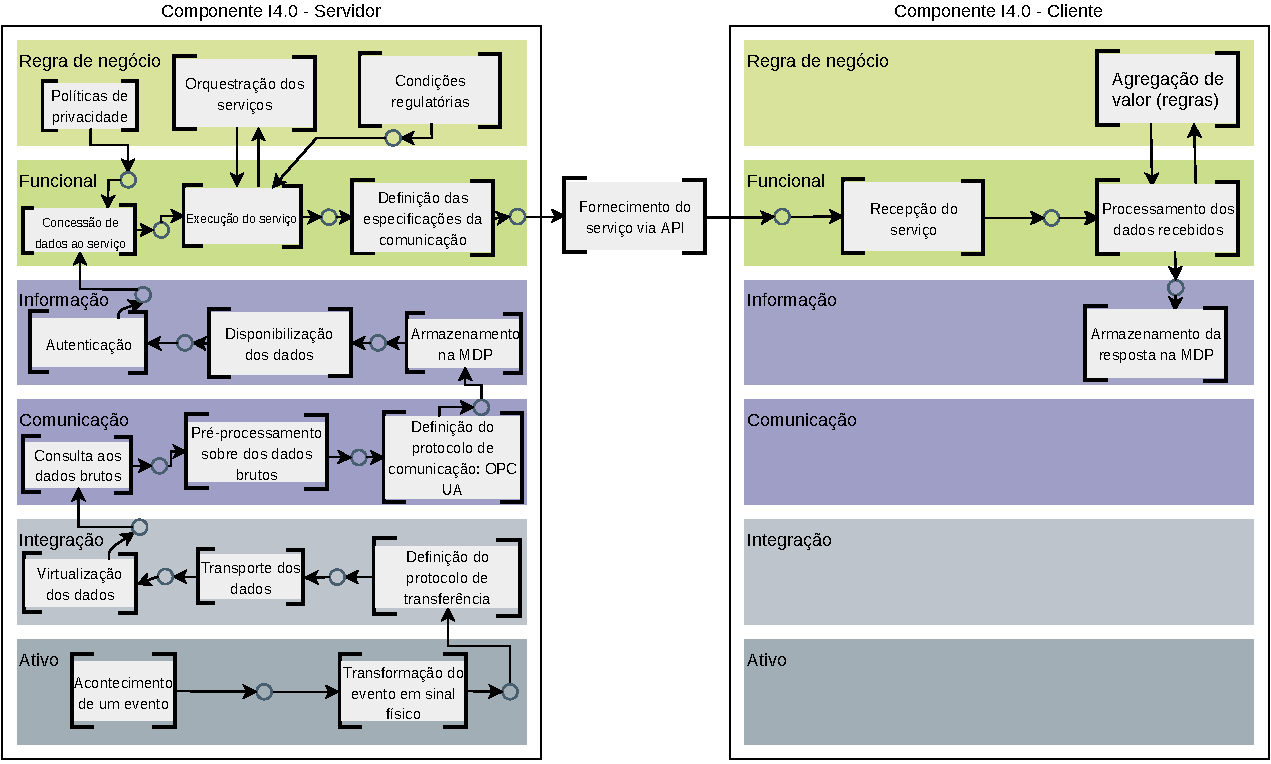
\includegraphics[width=1\textwidth]{rami-interacao}
		\fonte{O autor.}
	\end{figure}

	Esta operação começa com um evento físico no ativo, esta informação deve percorrer um fluxo padrão para que seja disponibilizada ao cliente por meio de um serviço. Este fluxo de atividades detalhado é apresentado a seguir:
	
	\begin{enumerate}
		\item Um evento físico acontece no mundo real acontece com o ativo.
		\item O evento é transformado em sinais físicos que são processados digitalmente.
		\item Já na camada de Integração, é definido o meio de transporte um procolo de transferência para o transporte dos sinais físicos como, por exemplo, o Wi-Fi, Ethernet, 5G, etc.
		\item Os dados são devidamente transportados pelo meio e protocolo definidos na atividade anterior até uma central de processamento.
		\item Os dados são processados e virtualizados. Nesta fase é criado um correspondente virtual para o evento do ativo físico, ou seja, os dados são digitalizados e enviados ao AAS.
		\item Os dados chegam à camada de Comunicação por meio de uma consulta aos dados de sinais já digitalizados.
		\item Os dados são então pré-processados, parte na qual é executada a limpeza dos dados, remoção de redundâncias e melhor os dados são reestruturados para serem armazenados na MDP.
		\item É definido o protocolo de comunicação padrão da Indústria 4.0: O OPC UA.
		\item Os dados são então enviados à camada de Informação, onde são salvos na MDP.
		\item Os dados são disponibilizados para consulta (após autenticação).
		\item É feita a autenticação para a determinação sobre quais dados o serviço solicitante pode ter acesso.
		\item O serviço, já autenticado, recebe os dados na camada funcional. A concessão de dados a um determinado serviço é feita segundo as políticas de privacidade contidas nas regras de negócio.
		\item Já de posse dos dados, o serviço é executado e a resposta para tal serviço é gerada. Todo o fluxo de informações desde o ativo até a camada funcional é mapeado para um serviço que tem como objetivo o compartilhamento de informações do ativo ao longo da cadeia de suprimentos, porém se aplica a qualquer outro serviço que necessite de informações em tempo real do ativo. Os serviços são orquestrados por um orquestrador de serviços e regido pelas condições regulatórias pertencentes à camada de regra de negócio.
		\item Após a geração da resposta do serviço, é feita a definição das especificações de comunicação, onde se estabelece o protocolo de comunicação a ser adotado na API (e.g., HTTP, MQTT), assim como o tipo de arquitetura (e.g., REST, SOAP) e o formato de intercâmbio (e.g., json, xml, yaml).
		\item A resposta do serviço (fornecimento do serviço) é enviada via API, definida com as especificações da comunicação.
		\item O Componente I4.0 do cliente recebe a resposta do serviço.
		\item A resposta é processada segundo as regras de agregação de valor estabelecidas na regra de negócio.
		\item Opcionalmente a resposta e/ou resultados de processamento da resposta podem ser salvos na MDP do Componente I4.0 do cliente ou descartados.
	\end{enumerate}
